\documentclass[12pt]{article}
\usepackage{authblk}

\usepackage{graphicx}
\usepackage{dcolumn}% Align table columns on decimal point
\usepackage{amsmath,amssymb}
\usepackage{bm}% bold math
\usepackage{enumitem}
\usepackage{float}

\usepackage{hyperref}
\hypersetup{
    colorlinks=true,
    linkcolor=blue,
    filecolor=magenta,      
    urlcolor=cyan,
}

\usepackage{afterpage}
\setlength\parindent{0pt}

\title{\Huge Multi-class classification on gene expression data}
\author[1]{Riccardo Castelli}
\author[2]{Simone Daniotti}

\affil[1]{Informatics Department, University of Milan}
\affil[2]{Physics Department, University of Milan}
\date{September 26, 2019}                    
\setcounter{Maxaffil}{0}
\renewcommand\Affilfont{\itshape\small}


\begin{document}

 \maketitle
  

\begin{abstract}
Many recent studies focused their attention to the relationship between gene expression and cancer types \cite{wang2018gene}. The goal of our work is to build learning algorithms that can classify cancer types starting from gene expression levels of patients. In doing so, we analysed the efficiency and computational performances of the most famous Python libraries that enable developers to build such models. \\
Full code available on GitHub at \cite{project}.
\end{abstract}


\newpage
\tableofcontents

\newpage
\section{Dataset description}

The dataset for this work is taken from the UCI Machine Learning Repo \cite{repo}, and it is part of the RNA-Seq (HiSeq, a tool for measuring gene expression levels) PANCAN dataset. The dataset is a collection of gene expression levels of patients having different types of tumor: BRCA (breast), KIRC (kidney), COAD (colon), LUAD (lung) and PRAD (prostate).
These data represent the quantity of gene information used in the synthesis of a functional gene product. 
For further information, we refer to \cite{weinstein2013cancer}.


\section{Dataset Manipulation}


\subsection{Preliminary manipulation}
Both dataset and labels can be downloaded in a .csv (comma separated value) format, that then can be easily imported into a Pandas Dataframe \cite{pandas}. The first column, which represents the patient's ID has been removed as it is useless for our purposes.


\subsection{Label handling}
The labels are strings representing the five types of cancer. Learning models can be created using raw features, as in the case of trees and forests, Label Encoding or One-Hot Encoding.
Label Encoding creates a map between the strings representing the categories and an ordered sequence of natural numbers, in our case from 0 to 4.
One-Hot Encoding creates a single binary label for each class, where the only 1 present in the vector represents the index of the class the example is associated with.  


\subsection{Normalization}
We normalized our dataset using the $normalize$ method present in Scikit-learn library $preprocessing$: this method scales vectors individually to unit norm. 


\subsection{Train and Test Set}

For training the models and evaluate them, we split the dataset into training and test set using the Scikit-learn method \cite{sk} $train\_test\_split$ from the $model\_selection$ library. Here we set the seed of the random split (for reproducibility purposes) and the proportions between the two sets: test set is the 15\% of our entire examples.


\subsection{Class Weighting}
Since our dataset is unbalanced, we chose to handle this problem using $class\_weight$ parameter (which is present in almost every classifier). This parameter can be defined as a dictionary that maps each class in the dataset with its respective weight; weights can be computed using Scikit-learn method $compute\_class\_weight$ in the $class\_weight$ library, which assigns greater values to the less represented classes. Through this parameter, the classifier is aware of the fact that some classes are more represented than others and gives the examples different importance during the training step.


\newpage
\section{Models}
We thought it could be a useful idea to approach our problem with relatively simple and more mathematically defined models, such as the Decision Trees, Random Forests and Support Vector Machines, and after their evaluation deepen in more complex ones, such as the Neural Networks. 
There are lots of books reviewing these architectures and concepts. Here we refer to \cite{geron2017hands} , \cite{bishop2006pattern} \cite{hertz1991introduction}.


\subsection{Decision Tree Classifier and Random Forests}

Decision Trees are versatile Machine Learning algorithms that can perform both classification and regression tasks, and even multi-output tasks. They are particularly useful for treating with complex data, such as a dataset that can hardly be represented by a vector in a multi-dimensional space.
Tree Classifiers have the structure of an ordered and rooted tree. It is ordered because the children of any internal node are numbered consecutively, and rooted because the splitting starts from only one node.
From that node, the model is built following the attribute selection measure.
Attribute selection measure is a heuristic for selecting the splitting criterion that partitions data in the best possible manner.


\begin{figure}[h!]
\centering
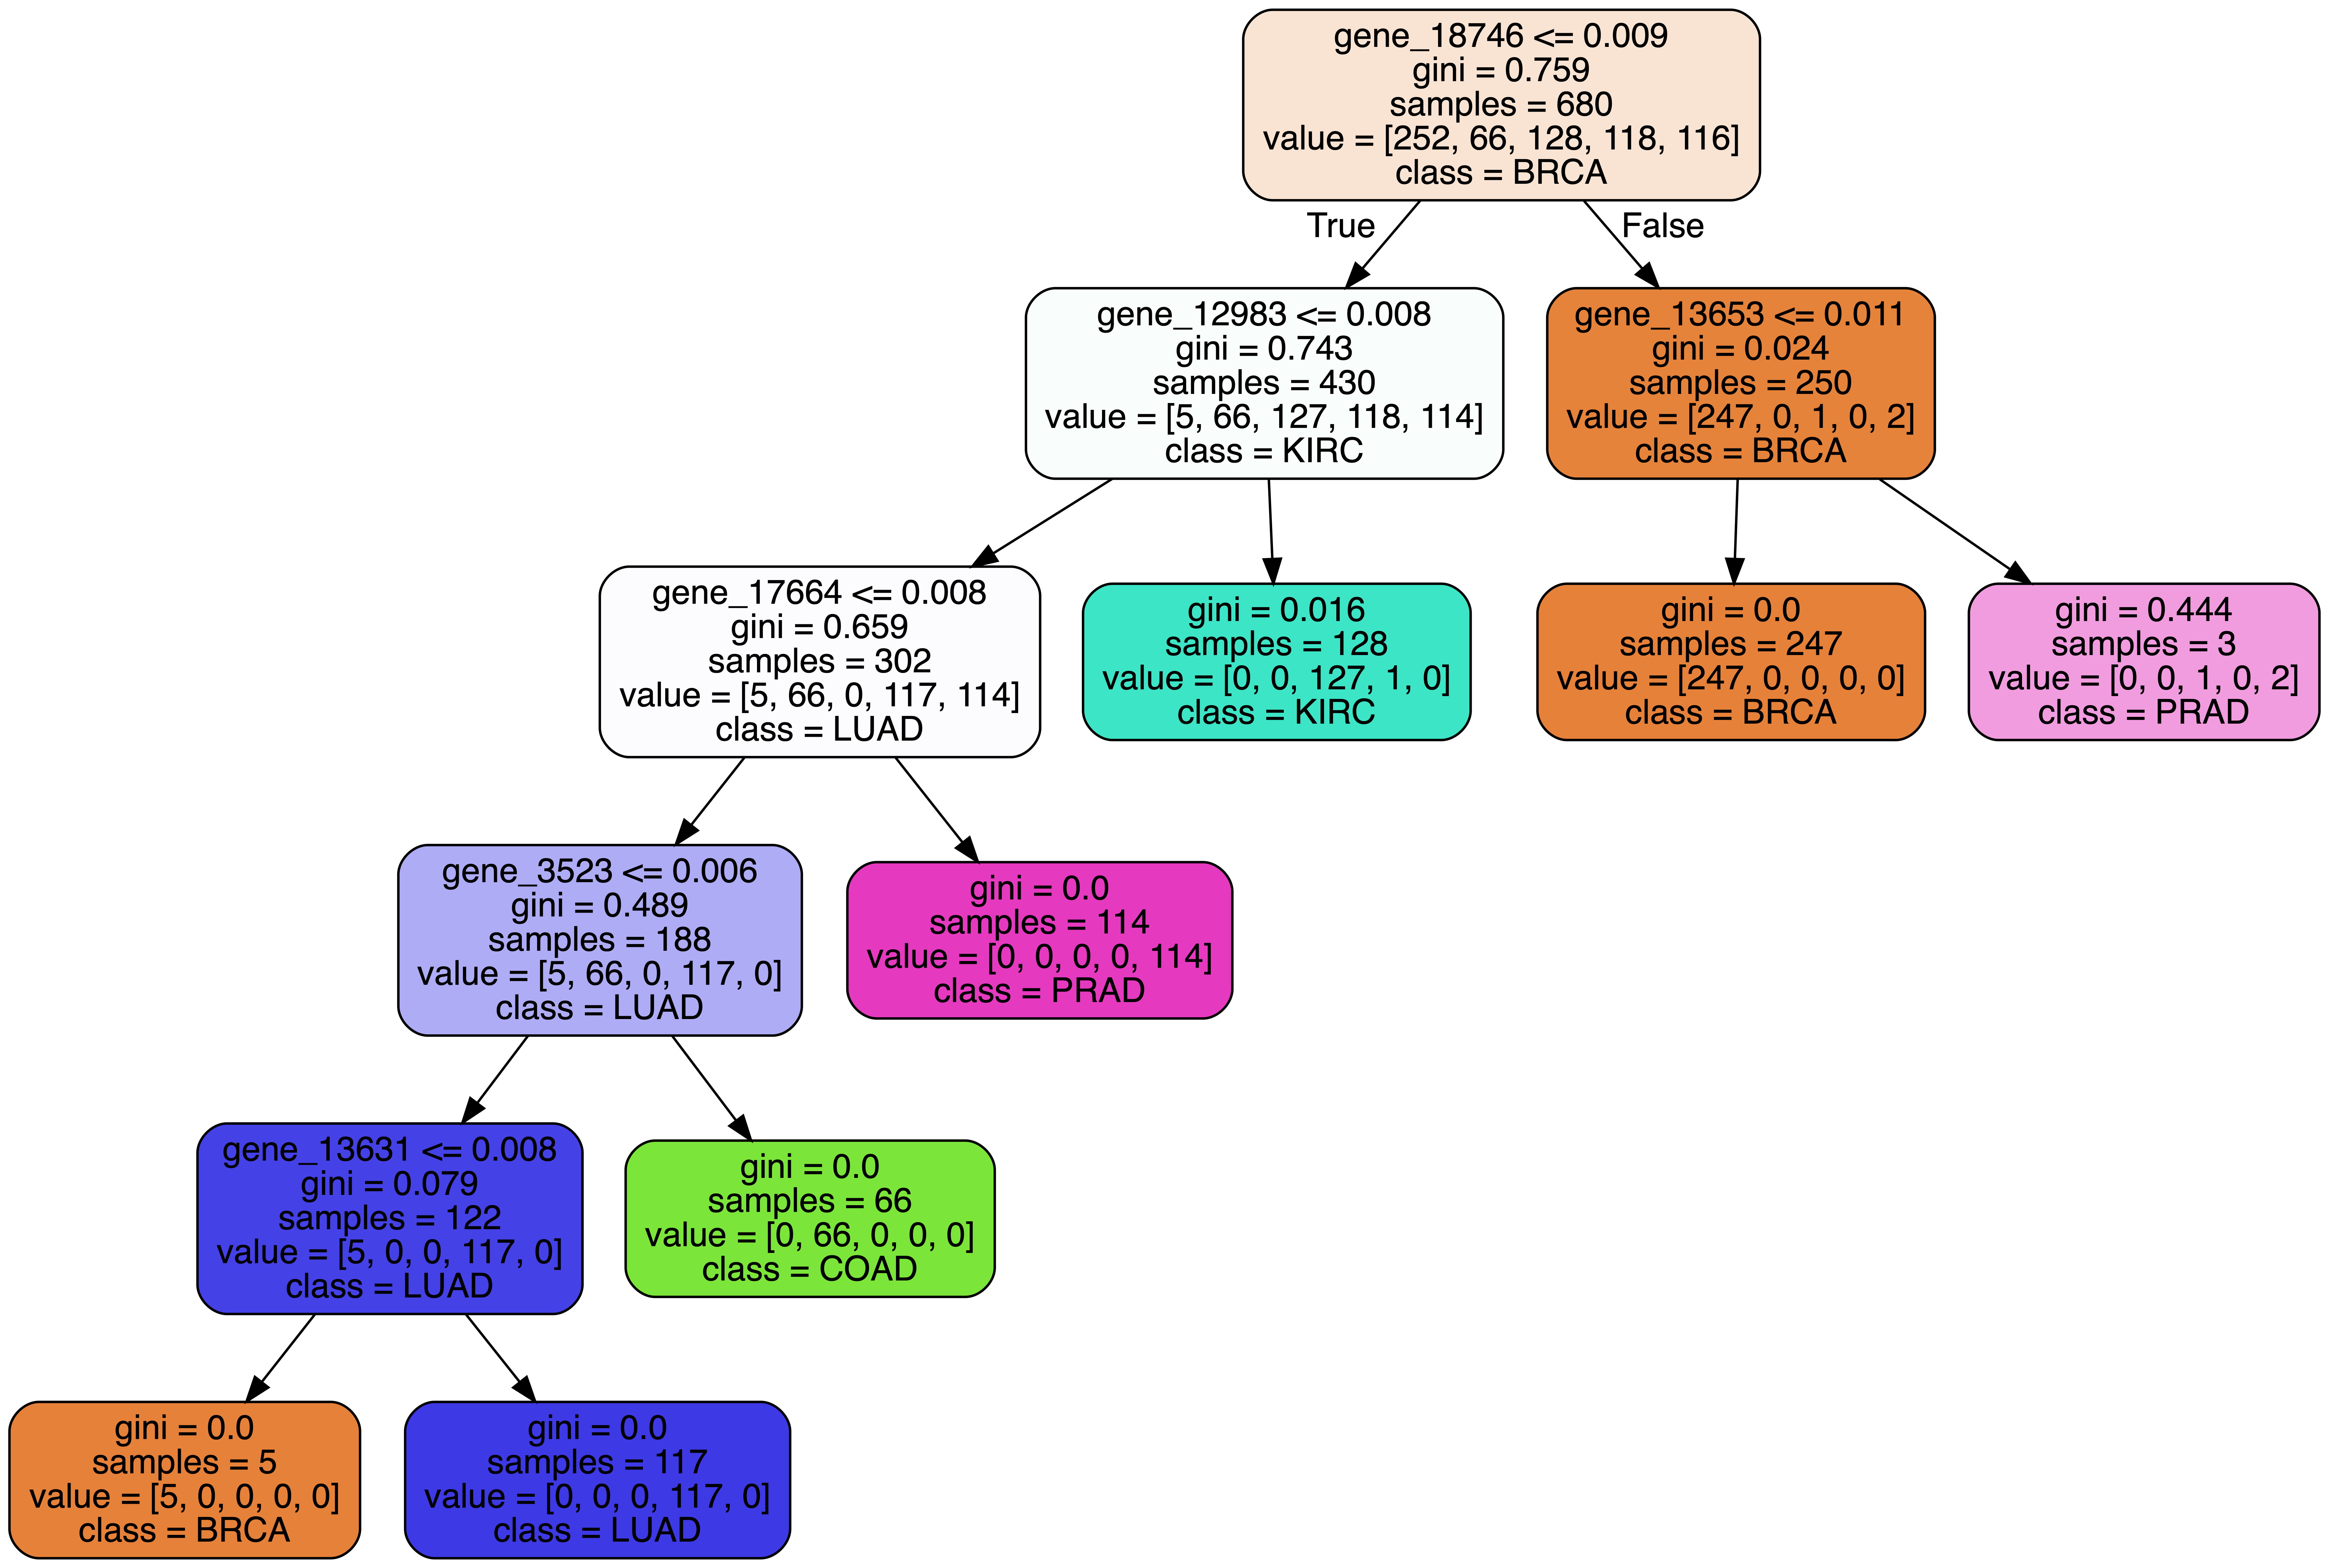
\includegraphics[width=\linewidth]{img/tree_best.png}
\caption{Shape of a tree classifier with tuned hyperparameters}
\label{fig1}
\end{figure}


Scikit-learn uses the Classification And Regression Tree (CART) algorithm to train Decision Trees. It works as follows: it firstly splits the training set in two subsets using a single feature $k$ and a threshold $t_k$ ; to choose $k$ and $t_k$, it searches for the pair $(k, t_k)$ that produces the purest subsets. The cost functions that the algorithm tries to minimize are different: the most used are Gini Impurity and Entropy, which are tunable in Scikit-learn by the $criterion$ hyperparameter; the $entropy$ hyperparameter measures Shannon's Entropy, a concept taken from the Information Theory. After the first split, the algorithm goes on until a stopping criterion is satisfied (for example the error is minimized). Each leaf of the tree corresponds to a possible classification label.

The aggregation of a group of predictors (regulated by certain rules, such as a majority rule) will often get better results than the best individual one. A group of predictors is called an ensemble, thus, this technique is called Ensemble Learning and an ensemble learning algorithm is called an ensemble method.
Training a group of Decision Tree Classifiers and gathering them into one single predictor is called a Random Forest.
The Random Forest algorithm introduces extra randomness when growing trees: instead of searching for the very best feature when splitting a node (as in the tree case), it searches for the best feature among a random subset of features, resulting in a greater tree diversity.


\subsection{Support Vector Machines (SVM)}
Another approach that we used to create a model that well classifies our dataset is the Support Vector Machines (SVM in short). Both a binary and a multi-class classifier, SVM tries to find the hyperplane (called decision boundary) that best separates the data. The optimal hyperplane is chosen by the use of the so called \textit{support vectors}, which are the samples of each class closest to the hyperplane. The distance between the support vectors is called $margin$, and the goal of the SVM is to maximise this margin in order to get a good separation of the classes in a way that also guarantees a good generalisation. 
SVM are particularly effective in high dimensional spaces, even when the number of features is greater than the number of samples: as this fact fits very well with the properties of our dataset, we decided to experiment the classification with this kind of model to see the results. \\
For the implementation, we utilised Scikit-learn SVC class from the svm library: for multi-class classification, it uses a “one-against-one” approach, creating $n\_class*(n\_class-1)/2$ (where $n\_class$ is the number of classes) classifiers and train each of them with two classes. \\
We considered three parameters for our model: $C$, $kernel$ and $class\_weights$. 
$C$ is called the ‘soft margin constant’: we can describe it as a measure of tolerance regarding the misclassification of the data, the more the C increases, the less amount of misclassified points the model will tolerate, giving them a huge penalty. During the training process, the model will try find a trade-off between the maximisation of the margin and the minimisation of the misclassification. 
$Kernel$ is used by the SVM to apply transformations to the data in order to project them in a higher dimensional space where they are more likely to be separable; this method, called the “kernel trick” is used to find non-linear decision boundaries. \\
The parameter $class\_weights$ is used to make the SVM aware that the dataset is unbalanced. 


\subsection{Deep Learning}
Moving to more complex models, we decided to implement a Deep Neural Network using Keras and Pytorch. In this section we will discuss about the peculiarity of these libraries and in the following we will provide the characteristics of our model, presenting his architecture and the losses and the optimizers we used.   

\subsubsection{Keras}
Keras \cite{keras} is a Python high-level machine learning library capable of running on top of multiple back-ends (such as TensorFlow, Theano, CNTK and many more), taking advantage of their power but putting aside their complexity. In fact, Keras allows the user to build deep learning models through a long list of modules that can be selected and combined in a very easy to use manner, which does not however comes at the expenses of the flexibility of the back-end frameworks and does not limit the user during the development and implementation process. 
The main Keras model is the Sequential, which is a linear stack of layers. The construction of the model requires three main phases: adding layers, compile the model and train it. 
In the first phase we can add an arbitrary number of layers using the $add$ function. There is a consistent number of type of layers that can be selected, for example, in our model, we chose to use 3 Dense (that is fully-connected) layers and 3 Dropout layers for regularization purposes. 
The second phase is where the model is compiled through the $compile$ function; this function needs the optimizer, the loss function and the metrics of evaluation to be specified. 
The third and last phase is the training of the model: Keras uses the $fit$ function for this purpose, to which we have to pass for example (other than the training examples and labels) the batch size, the epochs and the class weights. 
After the model has been built and trained, it can be evaluated on the test set using Keras’ method $evaluate$.


\subsubsection{PyTorch}
PyTorch \cite{torch} is a Python machine learning library, built to create learning algorithms based on graph models. 
It starts at low-level, but it has a lot of high-level APIs that allow to create even complex neural networks with a very few lines of code.
Its core element are Pytorch tensors, in the same way arrays are for Numpy, but built to take advantage of GPU computing.
The transition between low-level programming and APIs is truly continuous, which is a very important feature when it comes to build and tune a deep neural network.
In depth, PyTorch has some useful built-in methods to handle training and evaluation, for example $autograd$ to compute gradients and $DataLoader$ to handle training and batch loading.

\subsection{Neural network architecture, losses and optimizers}



\subsubsection{Architecture}
Our model is a fully connected linear deep neural network, composed by:

\begin{itemize}
\item an input layer of the size of the training set features;
\item $1_{st}$ hidden layer with 50 nodes;
\item $2_{nd}$ hidden layer with 25 nodes;
\item $3_{rd}$ hidden layer with 10 nodes;
\item an output layer with 5 nodes.
\end{itemize}
Between each layer has been applied a dropout of $20\%$ (during the weight update in the training step each neuron can be ignored with a probability of 0.2) and a ReLU activation function. Moreover, the net has been trained for 300 epochs, with a batch size of 16.


\subsubsection{Losses}
Here we list the losses used during our work:

\begin{description}[align=left]

\item [BCEWithLogitsLoss:] This loss combines in one single class both a Sigmoid layer and the BCELoss. This version is more numerically stable than using a plain Sigmoid followed by a BCELoss as, by combining the operations into one layer, we take advantage of the log-sum-exp trick for numerical stability. The equation of the loss is the following:

\begin{equation}
loss(x,y) = \mathbb{E} \left[ \{ l_1,....,l_N\} ^\top \right] , 
\end{equation}
where
\begin{equation}
l_{n} = - w_{n} \left[ y_{n}  \log[\sigma(x_{n}) + (1-y_{n})  \log(1 - \sigma(x_{n})) \right]
\end{equation}

\item [CrossEntropyLoss:] This criterion combines a $LogSoftmax$ and $NLLLoss$ in one single class. This criterion expects as the target of each value of the minibatch-sized 1D tensor a class index in the range [0,C-1]. The equation of the loss is the following:

\begin{equation}
loss(x,class) = - \log\left(\frac{\exp(x[class])}{\sum_{j}{\exp(x[j])}}\right)
\end{equation}

\end{description}


\subsubsection{Optimizers}
Optimization algorithms are used to minimise the loss function, in order to find optimum values for our learnable model’s parameter. During our neural network design and implementation we focused particularly on two main optimization techniques: Gradient Descent and Adam. \\ \\
\textbf{Gradient Descent}, one of the most famous and used optimization algorithms  \cite{hertz1991introduction}, works as follows: on each iteration, the algorithm computes the gradient of the loss function for the current weights values and updates them by an arbitrary percent (that we are able to choose by a parameter called learning rate); this procedure goes on util a stopping criterion is satisfied. 
The traditional algorithm needs to see the whole dataset in order to perform a parameter update, and this can lead to very slow computational times, so from this original idea it has been developed the Stochastic Gradient Descent, that updates the parameter for each training example, but since this approach can lead to fluctuations and difficulties in the convergence, an additional improvement named Mini Batch Gradient Descent was created, which solves a lot of issues related to GD and SGD performing a parameter update for every batch (a subset of training examples that we can decide the size of). 
For our model we implemented Mini Batch Gradient Descent, that takes as parameters the learning rate, which is variable through the decay rate, the Momentum (which accelerates the movement towards relevant directions) and the Nesterov (which makes the SGD perform the updates based on the previous momentum, in order to try to prevent to jump over minima due to the extreme acceleration of the descent).  \\
The formula is the following: \\ \\

\textit{For every mini batch of size n, repeat until convergence:} 
\begin{align*}
\nu_{t}  \gets \gamma  *  \nu_{t-1} - \alpha \nabla_{w} L(w - \gamma\nu_{t-1}), \\
w \gets  w - \nu_{t},
\end{align*}


where $\nu_{t}$ is the Momentum update calculated at time $t$, $\gamma$ is the Momentum term, $\eta$ is the learning rate and $\nabla_{w}$ is the gradient of $L$.   \\ \\
For our model, we chose a learning rate of 0.01, a decay rate of 0 and a Momentum term of 0.9. \\

Although we obtained very good result using this version of the SGD, we also decided to use another optimizer to compare the results. We chose to use \textbf{Adam} \cite{kingma2014adam}, a technique derived both from the idea of Momentum and another optimization algorithm called RMSProp. \\
While RMSProp tries to dampen oscillations by updating each parameter separately and choosing for each one a different learning rate computed using the exponential average of squares of gradients, Adam uses in addition the exponential average of gradients, keeping also two constants named $\beta_{1}$ and $\beta_{2}$ to control the decay rates of these two moving averages. \\
The formula is the following: \\ 


\textit{For each parameter $w^{j}$}: 
\begin{align*}
\nu_{t}  = \beta_{1}  *  \nu_{t-1} - (1 - \beta_{1}) *g_{t} \\
s_{t} =  \beta_{2} * s_{t-1} - (1-\beta_{2}) * g_{t}^2\\
\Delta w_{t} = -\eta \frac{\nu_{t}}{\sqrt{s_{t} + \epsilon}}* g_{t}\\
w_{t+1} = w_{t} + \Delta w_{t},
\end{align*}

where $\eta$ is the initial learning rate, $g_{t}$ is the gradient at time t along $w^{j}$, $\nu_{t}$ is the exponential average of gradients along $w_{j}$, $s_{t}$ is the exponential average of squares of gradients along $w_{j}$ and $\beta_{1},\beta_{2}$ are hyperparameters. \\ \\
For our model, we chose an initial learning rate of 0.01, $beta_{1}$=0.9 and $beta_{2}$=0.999 (as suggested from the Adam paper) and an epsilon value (to prevent divisions by zero) of $10^{-8}$.

\newpage
\section{Parameter optimization and Validation}
Once having built a model, a developer must ensure that the model has a good generalising capacity. Often, a too fitted net fails to predict in test set: this behaviour is called overfitting.
In the sections below, we will review some of the techniques used to avoid this problem and some characteristics of the models we considered.


\subsection{Cross-Validation}
One may desire to have a technique to evaluate the generalisation performances of the model before testing it. An idea could be to split again the training set, and using a part of it to test the performances: this procedure is called Cross-Validation.
It works as follows: it randomly splits the training set into $k$ distinct subsets called folds, then it trains and evaluates the model $k$ times, each time picking a different fold as the test set and using the other $k-1$ for training.
This procedure is automatically implemented in a lot of libraries inside both the methods used to train the classifiers as well as in the evaluation ones; for example, in Keras it is sufficient to enable the shuffling of data and specify the percentage of the training set that we want to use as validation in order to implement this technique. In our work we also utilised the $StratifiedKFold$ method form the $model\_selection$ library, which has the property to preserve the percentage of samples for each class present in the training set.

\subsection{Grid Search and Random Search}
During the process of tuning hyperparameters for each algorithm, one can see that some of them influence overfitting more than others: selecting the right parameters is a tedious job if one does it by hand, and it can become almost impossible as the number of parameters increases.
Instead, it is possible to use for example Scikit-learn's GridSearchCV, that will calculate all the possible combinations of the hyperparameters given in input and return the best of all evaluated through cross-validation. 
The grid search approach is fine when we are exploring relatively few combinations, but when the hyperparameter search space is large, it is often preferable to use RandomizedSearchCV instead. This class is similar to the one we have just discussed, but it evaluates random values (taken from a probability distribution) for every parameter passed.
It is useful when we want to explore larger parts of the hyperparameter search space and also lighten the computation.
Both functions were used in our work, giving similar results in terms of performances.


\subsection{Architecture settings}
In general, when we build a model, we must determine which parameters mostly influence the performances and try to tune them in a way that we obtain the best predictions. By using the techniques considered above, we obtained some optimal parameters for every model we designed. 


\subsubsection{Decision Tree}

\begin{itemize}
\item Criterion for the splitting = gini
\item Maximum depth for a tree = 5
\item Maximum number of leaf nodes =7
\end{itemize}


\subsubsection{Random Forest}

\begin{itemize}
\item Criterion for the splitting = entropy. \\ (Some of them are inherited from Trees)
\item Number of trees in the forest = 60
\item Maximum number of leaf nodes = 50
\item Bootstrap samples are used when building trees. \\ (Otherwise, the whole datset is used to build each tree).
\end{itemize}

\subsubsection{Support Vector Machine}

\begin{itemize}
\item C = 10;
\item Kernel= linear
\end{itemize}
                            
\newpage
\section{Models Evaluation}


\subsection{Feature Selection and Dimensionality Reduction}
Our dataset is really interesting because while it is formed by a low number of patients (800) it has a really high number of features (more than 20000). To improve computation times, especially for training times, we tried out some dimensionality reduction techniques. Dimensionality reduction assumes an intrinsic dimension of the data significantly lower than the data space and tries to delete all the redundant or less useful information in order to obtain a vector with a lower number of components that maintain a considerably amount of information. In our work we used the Principal Component Analysis (PCA in short) and the Permutation Importance. \\ \\
The idea of the \textbf{Principal Component Analysis} algorithm is to find among all the possible directions in the space of data the one that maximise the variance once that the data are projected in that direction. We implemented  PCA using Scikit-learn PCA method from the decomposition library, setting the number of components to 700: the resulting features still retained a high percentage of information (98\%), but with a remarkable compression rate that reduced our data to slightly less than 4\%. \\ \\
Another procedure was to adopt the eli5 library \cite{pm} for computing \textbf{Permutation Importance}, that works as follows:
one at a time a feature is removed from the test part of the dataset and replaced it with random noise; then an evaluation score (depending on the model we developed) is computed. This method works if noise is drawn from the same distribution as the original feature values (as otherwise the estimator may fail) and the simplest way to get such noise is to shuffle values for a feature (i.e. use other examples' feature values). \\
We applied the permutation importance method to our tree classifier and got the results shown in Figure \ref{fig_perm}. \\


\begin{figure}[H]
\centering
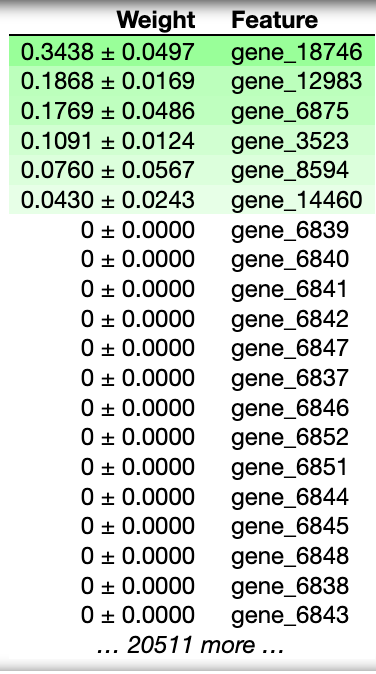
\includegraphics[width=0.2\textwidth]{img/perm}
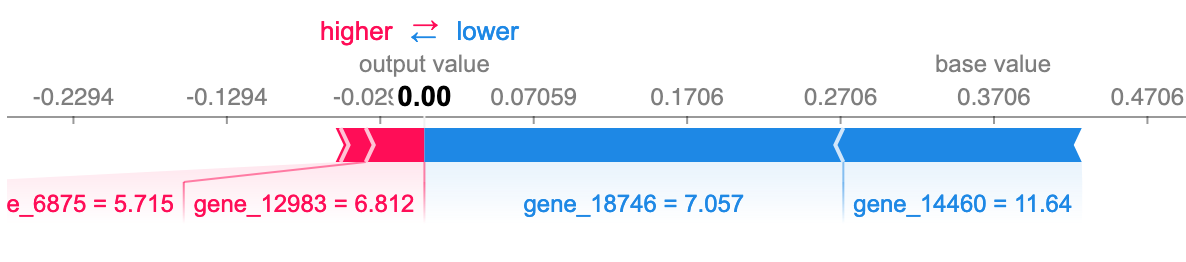
\includegraphics[width=0.77\textwidth]{img/shap.png}
\caption{On the left: permutation importance for the parameter tuned tree; it clearly shows that only a low number of genes is correlated with the prediction. On the right: a visual description using Shape library of how these features influence the data prediction.}
\label{fig_perm}
\end{figure}


From these results we assumed that only highlighted genes were responsible for the predictions, so we tried to train a Decision Tree Classifier keeping only those, reducing the features dimensionality from 20530 to 6. \\
The results are the shown in Figure \ref{fig_perm_m}.


\begin{figure}[h!]
\centering
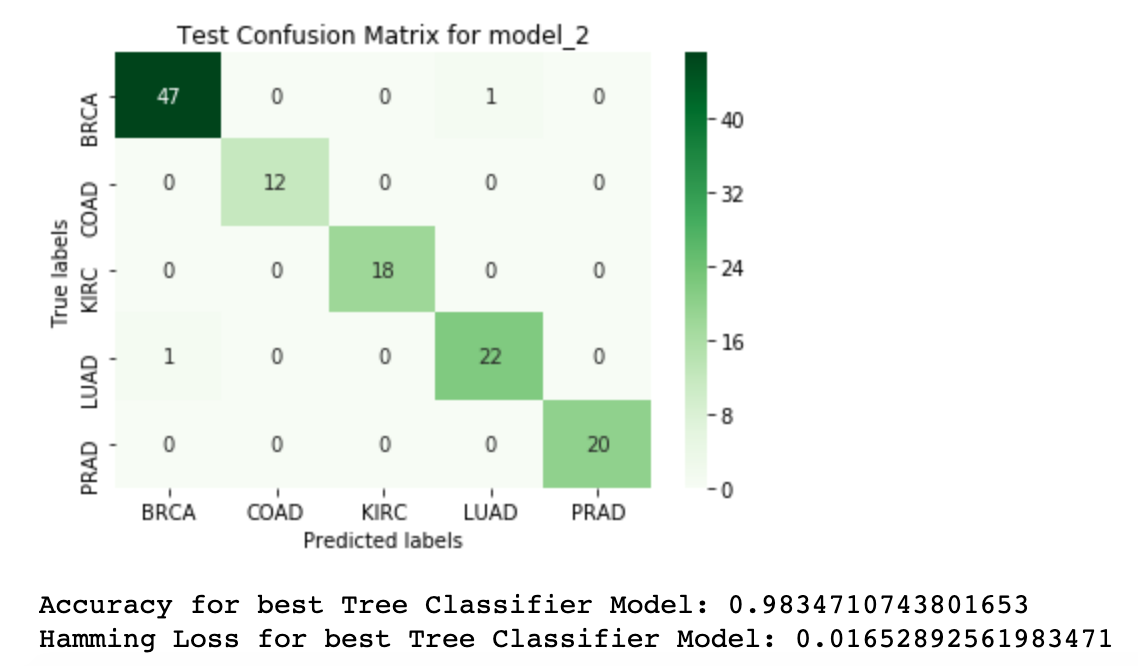
\includegraphics[width=120mm]{img/perm_matrix}
\caption{Confusion matrix and evaluation metrics for the tree classifier trained with only relevant genes.}
\label{fig_perm_m}
\end{figure}

\newpage
\subsection{Metrics}
During our analysis we used a variety of losses and metrics:

\begin{itemize}
\item Accuracy: in multi-class problems, this is a discrete measure of predictions, in the sense that results scores only when predition is exact.
\item Hamming Loss: the fraction of labels that are incorrectly predicted.
\end{itemize}

Talking about these metrics, we believe that they are not a truly good measures for the evaluation of the performances of models in the case of unbalanced classes. A more precise measure, and the metric we used the most during our work, is the Confusion Matrix. Having the true labels as rows and predictions as columns, the confusion matrix presents the number of right classifications on the principal diagonal and the sum of misclassifications off-diagonal. In the following section we will present our results.

\subsubsection{Models results}

\begin{itemize}
\item For the optimal Decision Tree Classifier, we have an Accuracy of $0.99174$ and a Hamming Loss of $0.00826$. The model was trained in $3.73$ seconds. 
The resulting confusion matrix is shown in Figure \ref{fig_treeandforest}. 

\item For the optimal Random Forest Classifier, we have and Accuracy of $1.0$ and a Hamming Loss of $0.0$. The model was trained in $2.37$ seconds. 
The resulting confusion matrix is shown in Figure \ref{fig_treeandforest}. 

\begin{figure}
\centering
\advance\leftskip-4cm
\advance\rightskip-4cm
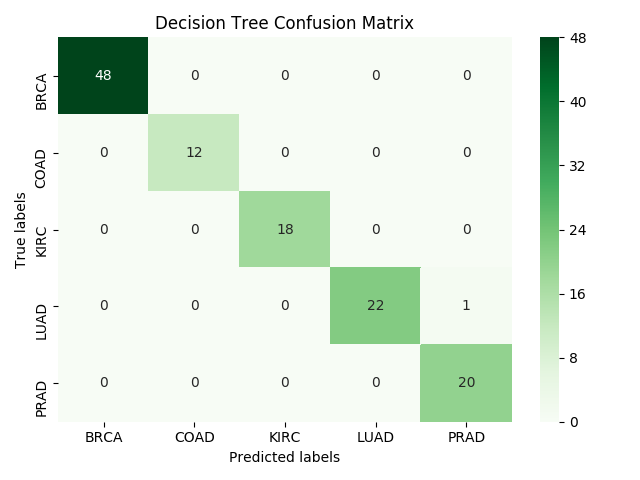
\includegraphics[width=0.60\textwidth]{img/dt.png}
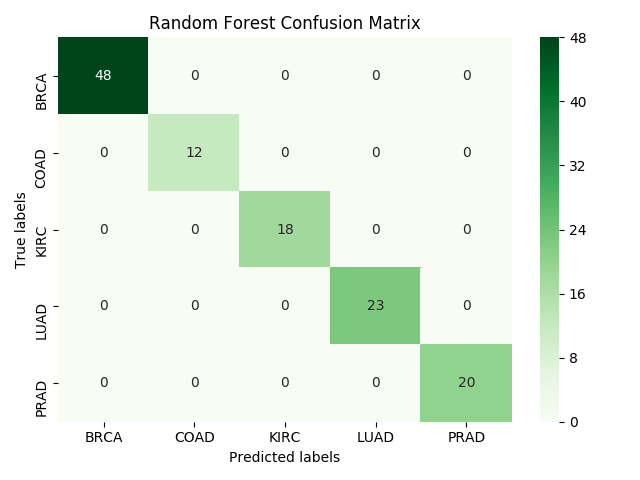
\includegraphics[width=0.60\textwidth]{img/rf.png}
\caption{On the left the confusion matrix for the Decision Tree; on the right the Random Forest one.}
\label{fig_treeandforest}
\end{figure}

\newpage
\item For the optimal Support Vector Machine, we have an Accuracy of $0.99705$. The model was trained in $0.1$ seconds.
The resulting confusion matrix is shown in Figure \ref{fig_svm}. 

\begin{figure}[h!]
\centering
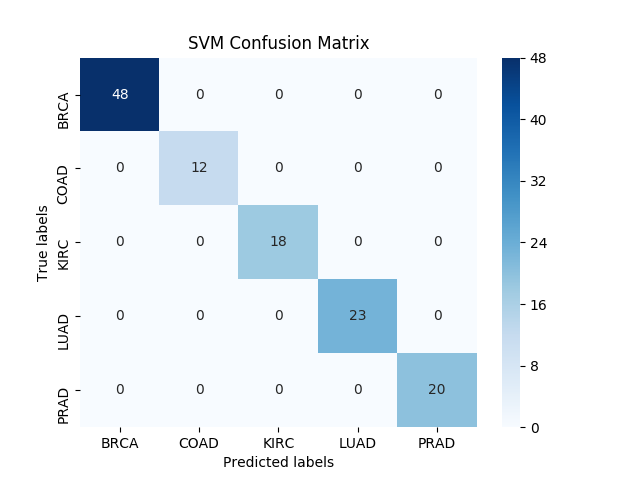
\includegraphics[width=100mm]{img/svm.png}
\caption{Confusion matrix for the optimal Support Vector Machine.}
\label{fig_svm}
\end{figure}

\begin{figure}
\centering
\advance\leftskip-4cm
\advance\rightskip-4cm
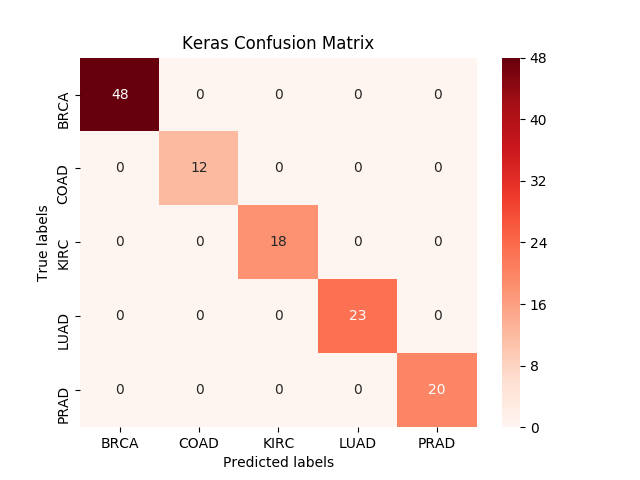
\includegraphics[width=0.60\textwidth]{img/keras.png}
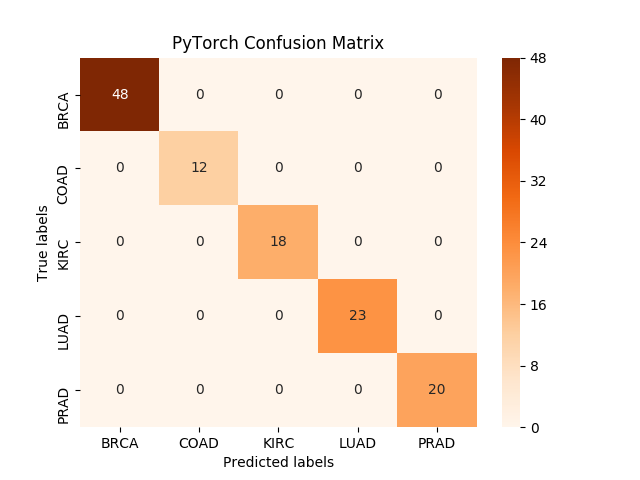
\includegraphics[width=0.60\textwidth]{img/pytorch.png} 
\caption{On the left the confusion matrix for the Keras Deep Neural Network with One-Hot encoded labels; on the left the Pytorch one (results for Label and One-Hot Encoding are the same).}
\label{fig_deep}
\end{figure}

\newpage
\item For the optimal Keras Deep Neural Network with One-Hot Encoding and CrossEntropyLoss, the model was trained in $25.52$ seconds, ending with a loss of the test set of $5,70688e-06$ and an Accuracy on the test set of $1.0$.
The resulting confusion matrix is shown in Figure \ref{fig_deep}. 

\item For the optimal PyTorch Deep Neural Network with Label Encoding and CrossEntropyLoss, the model was trained in $21.72$ seconds ending with a loss of $6,407e-07$. 
The resulting confusion matrix is shown in Figure \ref{fig_deep}.

\item For the optimal Pytorch Deep Neural Network with One-Hot Encoding and BCEWithLogitsLoss, the model was trained in $21.21$ seconds ending with a loss of $0,00543$. 
The resulting confusion matrix is shown in Figure \ref{fig_deep}.
\end{itemize}



\newpage
\section{Conclusions and Outlook}
After our evaluation, we can clearly see that all models can predict the task with an optimal precision value. \\
From our permutation importance procedure (and also from trees' and forests' structures) it is reasonable to confirm a correlation (but we can still not say anything about a causal relationship) between gene expression levels and a certain cancer type. \\
From our computation time analysis we can see a clear difference between the models: simpler models generally have times one or two orders of magnitude smaller than the deep learning ones. \\
Regarding the ease of development, Keras shows its true strength when fast building and simplicity of code is needed, while for a better understanding of the architecture and in depth parameter tuning is preferable to use Pytorch instead. \\ \\ 
For future improvements, it could be interesting to test our models using bigger datasets: this could be the right occasion to improve both their architectures and parameters. However, this requires a deeper analysis that was not needed for our goal, and for this reason we did not focus on it. \\
To enrich and improve our models comprehension and analysis, it could be an advantage to have a better integration between statistical and deep model building methods: for example, a good start could be using the Skorch \cite{skorch} library. \\
Moreover, as recent published articles show \cite{wang2018gene}, it could be interesting to focus more on the relationship between gene expression and cancer types.


\newpage
\bibliography{Bibliography}
\bibliographystyle{unsrt}


\end{document}